\begin{surferPage}[7-Eck]{Eine 7-Eck-symmetrische Septik}
  Diese einem Weihnachtsstern ähnelnde Fläche ist vom Grad $7$.  
    Bis vor Kurzem stellte sie noch die maximal bekannte Anzahl, $84$, von reellen
    Singularitäten auf einer Septik dar;
    erst 2004 hat Oliver Labs diesen Weltrekord auf $99$ verbessert. 

    Die jeweils drei Kissen, die bei der $7$-Eck-symmetrischen Septik (großes
    Bild) 
    übereinander liegen, kommen wie bei der 
    Chmutov Oktik (vorige Fläche) von der Verwendung der Tchebychev Polynome.
    Daher wundert es nicht, dass auch diese Fläche eine Variante von
    Chmutovs Flächen ist. 
    Hier wurde die ebene Kurve $T_d(x)+T_d(y)$
    durch ein regelmäßiges $7$-Eck $S_7(x,y)$ ersetzt:
    \[S_7(x,y) + \lambda \cdot T_d(z) = 0,\]
    für ein geeignetes $\lambda\in\RR$. 
    \vspace*{-0.3em}
    \begin{center}
      \begin{tabular}{c@{\qquad}c}
        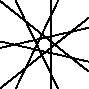
\includegraphics[height=1.5cm]{./../../common/images/labsseptic1.pdf}
        &
        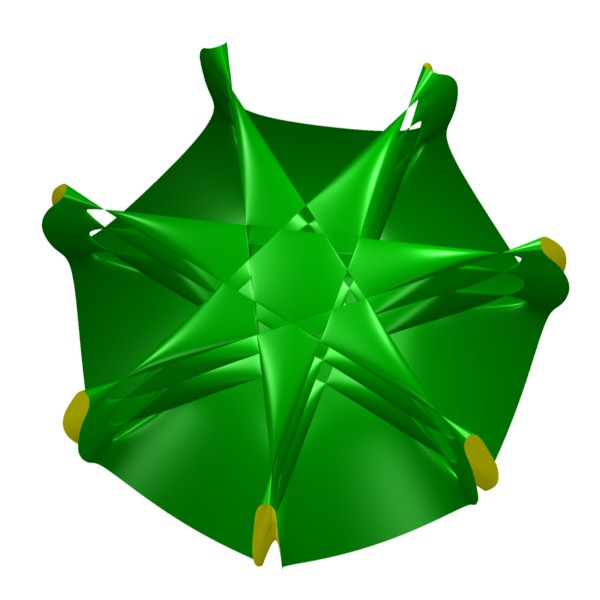
\includegraphics[height=1.5cm]{./../../common/images/septic_7eck_von_oben}
      \end{tabular}
    \end{center}
    \vspace*{-0.3em}    
   Diese Variante von Chmutovs Konstruktion stammt von Duco van
    Straten. 
\end{surferPage}
